%
% $RCSfile: agile_methodologies.tex,v $
%
% Copyright (C) 2002-2008. Christian Heller.
%
% Permission is granted to copy, distribute and/or modify this document
% under the terms of the GNU Free Documentation License, Version 1.1 or
% any later version published by the Free Software Foundation; with no
% Invariant Sections, with no Front-Cover Texts and with no Back-Cover
% Texts. A copy of the license is included in the section entitled
% "GNU Free Documentation License".
%
% http://www.cybop.net
% - Cybernetics Oriented Programming -
%
% http://www.resmedicinae.org
% - Information in Medicine -
%
% Version: $Revision: 1.1 $ $Date: 2008-08-19 20:41:05 $ $Author: christian $
% Authors: Christian Heller <christian.heller@tuxtax.de>
%

\section{Agile Methodologies}
\label{agile_methodologies_heading}
\index{Agile Methodologies}
\index{Agile Manifesto}
\index{Extreme Programming}
\index{XP}
\index{Open Source Software}
\index{OSS}
\index{Crystal Family}
\index{Adaptive Software Development}
\index{ASD}
\index{Scrum}
\index{Feature Driven Development}
\index{FDD}
\index{Dynamic System Development Method}
\index{DSDM}
\index{Context Driven Testing}
\index{Agile Alliance}

The principles of \emph{Agile Methodologies} (figure \ref{agile_figure}) are
applied by a group of so-called \emph{lightweight}, \emph{adaptive} software
development processes with few bureaucracy, less predictability, less process-
and document-orientation, but more emphasis on people and their skills, and on
source code -- which is considered the key part of documentation.

\begin{figure}[ht]
    \begin{center}
        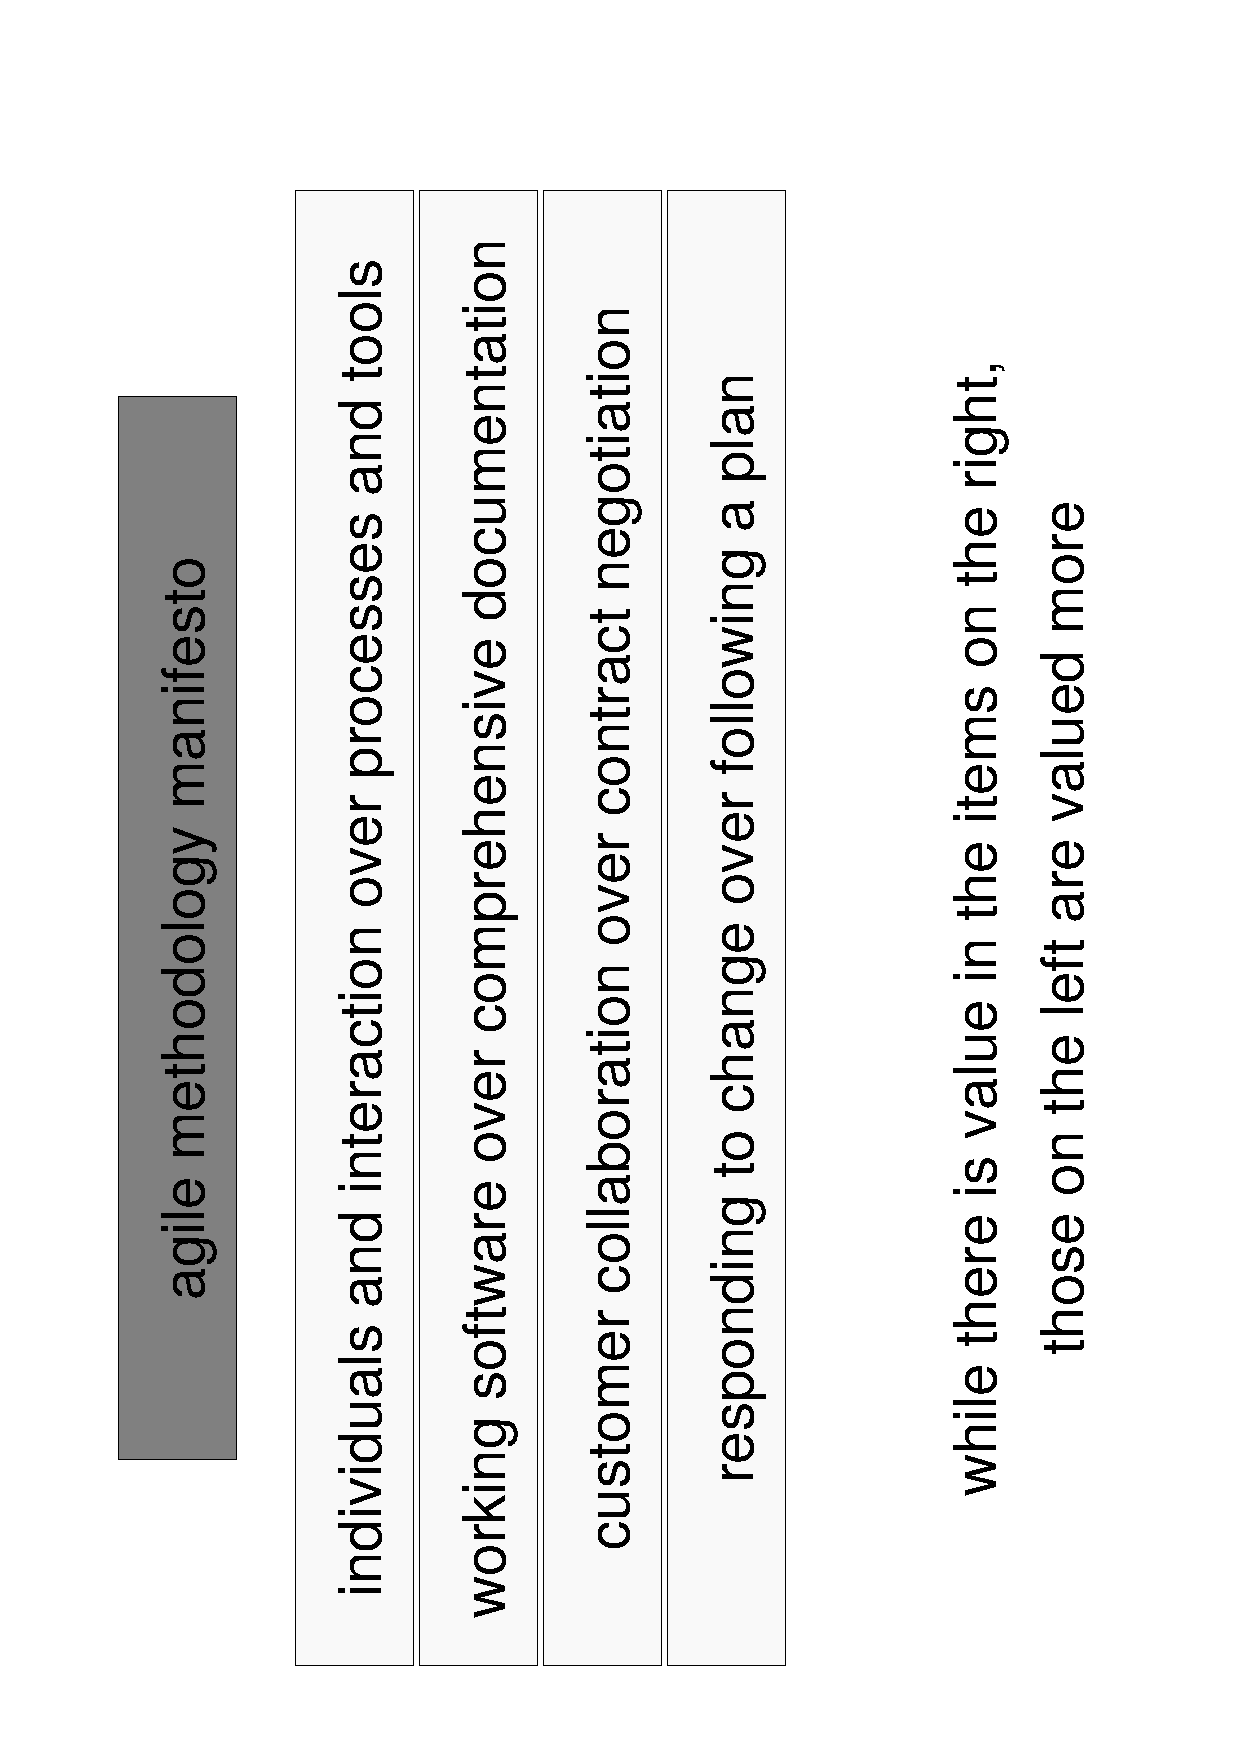
\includegraphics[scale=0.3,angle=-90]{graphic/agile.pdf}
        \caption{Agile Manifesto}
        \label{agile_figure}
    \end{center}
\end{figure}

Besides \emph{Extreme Programming} (XP) and \emph{Open Source Software} (OSS)
development, both described in section \ref{extreme_programming_heading}, there
are several other methodologies that fit under the \emph{Agile} banner. Fowler
explains some of them in \cite{fowlernewmethodology}, which contains Alistair
Cockburn's \emph{Crystal Family}, Jim Highsmith's
\emph{Adaptive Software Development} (ASD), \emph{Scrum},
\emph{Feature Driven Development} (FDD) by Jeff De Luca and Peter Coad, the
\emph{Dynamic System Development Method} (DSDM) specified by a consortium of
British companies and some remarks on \emph{Context Driven Testing}.

For the purpose of this paper, further investigation on details of the
mentioned methodologies is not needed. The general principles of agile software
development (manifesto) are the important part to recognise, because they
suggest a different, more \emph{agile} approach to software engineering.
Although many techniques of agile methodologies had been known and used for
long, at least in OSS development, they had not been investigated, documented
and promoted for business use in this form before. This is the great
achievement of the \emph{Agile Alliance} \cite{agilealliance}.
